% Standalone RAKL evidence-lane map (Paper II).
% Three lanes: objective known-world (established) | natural-domain (demoted) | future (planned).
% Build:  pdflatex evidence_lanes.tex  -> evidence_lanes.pdf
\documentclass[border=6pt]{standalone}
\usepackage{tikz}
\usepackage{helvet}\renewcommand{\familydefault}{\sfdefault}
\usetikzlibrary{positioning,arrows.meta,shapes.geometric,fit,backgrounds,calc}
\definecolor{oiblue}{RGB}{0,114,178}
\definecolor{oiverm}{RGB}{213,94,0}
\begin{document}
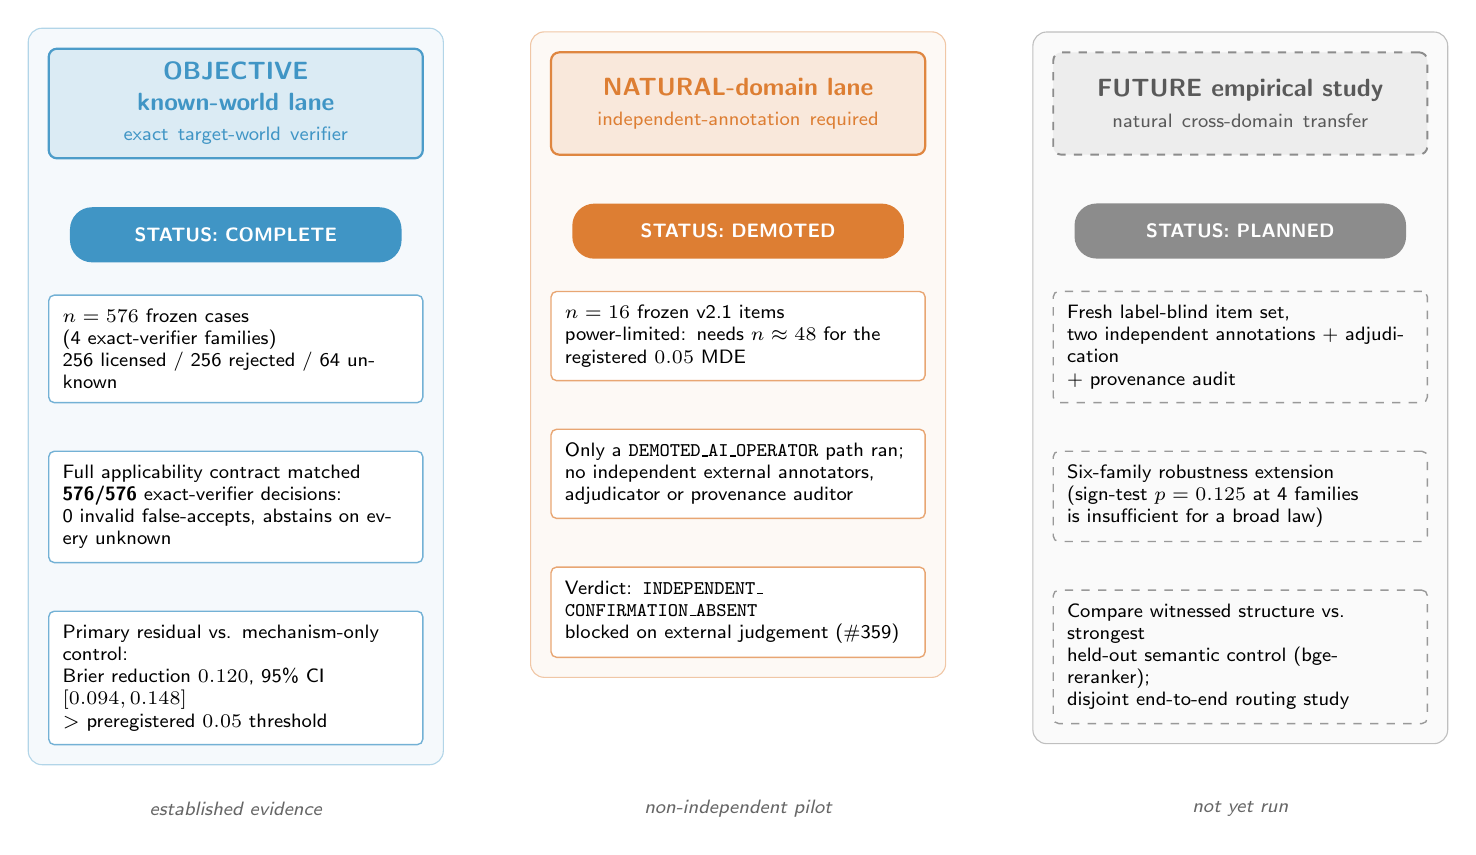
\begin{tikzpicture}[
  font=\small,
  >={Stealth[length=2.4mm]},
  head/.style={rounded corners=3pt, align=center, inner sep=5pt,
               minimum height=13mm, text width=44mm, font=\small\bfseries},
  item/.style={rounded corners=2pt, draw=black!45, line width=0.5pt, align=left,
               inner sep=5pt, text width=44mm, font=\scriptsize, fill=white},
  badge/.style={rounded corners=8pt, align=center, inner sep=3pt,
                minimum height=7mm, text width=40mm, font=\scriptsize\bfseries},
  node distance=6mm,
]

% ==================== LANE 1 : OBJECTIVE (established) ====================
\node[head, fill=oiblue!14, draw=oiblue!70, line width=0.8pt, text=oiblue!75]
   (h1) {OBJECTIVE known-world lane\\{\scriptsize\mdseries exact target-world verifier}};
\node[badge, below=of h1, fill=oiblue!75, text=white] (b1) {STATUS: COMPLETE};
\node[item, below=4mm of b1, draw=oiblue!55] (i1a)
  {$n=576$ frozen cases\\(4 exact-verifier families)\\256 licensed / 256 rejected / 64 unknown};
\node[item, below=of i1a, draw=oiblue!55] (i1b)
  {Full applicability contract matched\\ \textbf{576/576} exact-verifier decisions:\\
   0 invalid false-accepts, abstains on every unknown};
\node[item, below=of i1b, draw=oiblue!55] (i1c)
  {Primary residual vs. mechanism-only control:\\
   Brier reduction $0.120$, 95\% CI $[0.094,0.148]$\\
   $>$ preregistered $0.05$ threshold};

% ==================== LANE 2 : NATURAL (demoted) ====================
\node[head, right=16mm of h1, fill=oiverm!14, draw=oiverm!75, line width=0.8pt, text=oiverm!80]
   (h2) {NATURAL-domain lane\\{\scriptsize\mdseries independent-annotation required}};
\node[badge, below=of h2, fill=oiverm!80, text=white] (b2) {STATUS: DEMOTED};
\node[item, below=4mm of b2, draw=oiverm!55] (i2a)
  {$n=16$ frozen v2.1 items\\power-limited: needs $n\approx 48$ for the\\registered $0.05$ MDE};
\node[item, below=of i2a, draw=oiverm!55] (i2b)
  {Only a \texttt{DEMOTED\_AI\_OPERATOR} path ran;\\
   no independent external annotators,\\adjudicator or provenance auditor};
\node[item, below=of i2b, draw=oiverm!55] (i2c)
  {Verdict: \texttt{INDEPENDENT\_}\\ \texttt{CONFIRMATION\_ABSENT}\\
   blocked on external judgement (\#359)};

% ==================== LANE 3 : FUTURE (planned) ====================
\node[head, right=16mm of h2, fill=black!7, draw=black!45, line width=0.7pt,
      text=black!65, dashed] (h3)
   {FUTURE empirical study\\{\scriptsize\mdseries natural cross-domain transfer}};
\node[badge, below=of h3, fill=black!45, text=white] (b3) {STATUS: PLANNED};
\node[item, below=4mm of b3, draw=black!40, dashed, fill=black!2] (i3a)
  {Fresh label-blind item set,\\two independent annotations + adjudication\\ + provenance audit};
\node[item, below=of i3a, draw=black!40, dashed, fill=black!2] (i3b)
  {Six-family robustness extension\\(sign-test $p=0.125$ at 4 families\\is insufficient for a broad law)};
\node[item, below=of i3b, draw=black!40, dashed, fill=black!2] (i3c)
  {Compare witnessed structure vs. strongest\\
   held-out semantic control (bge-reranker);\\
   disjoint end-to-end routing study};

% ==================== lane background frames ====================
\begin{scope}[on background layer]
  \node[draw=oiblue!30, rounded corners=5pt, fill=oiblue!4,
        fit=(h1)(i1c), inner sep=7pt] {};
  \node[draw=oiverm!35, rounded corners=5pt, fill=oiverm!4,
        fit=(h2)(i2c), inner sep=7pt] {};
  \node[draw=black!25, rounded corners=5pt, fill=black!2,
        fit=(h3)(i3c), inner sep=7pt] {};
\end{scope}

% ==================== established vs pending divider caption ====================
\node[font=\scriptsize\itshape, text=black!60, align=center, below=6mm of i1c.south -| h1]
   (cap1) {established evidence};
\node[font=\scriptsize\itshape, text=black!60, align=center] at (cap1 -| i2c)
   {non-independent pilot};
\node[font=\scriptsize\itshape, text=black!60, align=center] at (cap1 -| i3c)
   {not yet run};

\end{tikzpicture}
\end{document}
